\documentclass[]{article}
\usepackage{graphicx}
\usepackage{float}
\graphicspath{ {images/} }
\usepackage{hyperref}
\hypersetup{
	colorlinks=true,
	linkcolor=blue,
	filecolor=magenta,      
	urlcolor=cyan,
	pdftitle={Overleaf Example},
	pdfpagemode=FullScreen,
}
%opening
\begin{document}

\title {Data analysis}
\author {Maarten Donkersloot}
\date{\today}


\maketitle

\newpage

\section{Introduction}
To better understand our data and use it in meaningful ways we did a data analysis on the most important columnsw. 

\section {Data gathering}
Our data was sourced from \href{https://github.com/IoTsec/Room-Climate-Datasets}{an already existing study}, with our own generate acceptability columns using the \href{https://www.researchgate.net/figure/ASHRAE-55-limits-for-thermal-Comfort-adapted-from-ASHRAE-55-2017_fig5_327597687}{ASHREA 55 standard}.

\section{Data explanation}
\begin{itemize}
\item  original-entry-id: Data is concatenated from multiple days/rooms, these are the original entry id's from those sources.
\item  node-id: At what place in the room the data was collected from
\item  room: Which room was used to take the reading 
\item  datetime: datetime of reading
\item  relative-time: The time between this and the previous reading
\item  date: Date of reading
\item  temperature: Temperature in Celsius
\item  mean-temp-day: The mean temperature from the day of the reading in Mannheim Germany (place where the study took place)
\item  heatindex: What the temperature feels like
\item  relative-humidity: Percentage of humidity in the air
\item  light-sensor-one-wavelength: Wavelength in nm at reading time
\item  light-sensor-two-wavelength: Wavelength in nm at reading time
\item  number-occupants: Amount of people in the room at the time of the reading
\item  activity-occupants: Activity the occupants were doing at the time off the reading  (0 = n/a, 1 = read, 2 = stand, 3 = walk, 4 = work)
\item  door-state: Was the door open or closed
\item  window-state: was the window open or closed
\item  tmp-cmf: Comfort temperature a that specific running mean temperature, in °C
\item  tmp-cmf-80-low: Lower acceptable comfort temperature for 80\% occupants, in °C
\item  tmp-cmf-80-up: Upper acceptable comfort temperature for 80\% occupants, in °C
\item  tmp-cmf-90-low: Lower acceptable comfort temperature for 90\% occupants, in °C
\item  tmp-cmf-90-up: Upper acceptable comfort temperature for 90\% occupants, in °C
\item  acceptability-80: Acceptability for 80\% occupants
\item  acceptability-90: Acceptability for 90\% occupants
\end{itemize}
\section{Univariate analysis}
First we wanted to do a univariate analysis to get a better understanding of the individual features.

\subsection{Feature: Room}
We found that the room feature is positively skewed towards A making room C less prominent in the dataset.
\begin{figure}[H]
	\centering
	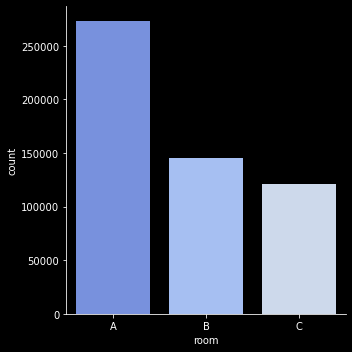
\includegraphics[width=0.90\textwidth]{univariate_1.png}
	\caption{Record count per room}
\end{figure}

\subsection{Feature: Date}
We found that the Date feature is positively skewed towards 2016. 2017 makes up 23 percent off all data. Including 2017 may lead to potential overfitting.


\begin{figure}[H]
	\centering
	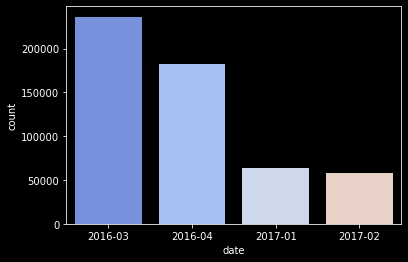
\includegraphics[width=0.90\textwidth]{univariate_2.png}
	\caption{Record count per month}
\end{figure}



\subsection{Feature: Temperature}
We found that the Temperature feature has overfitting towards the upper end of the dataset, we don't know where this comes from yet and will investigate this further in the multivariate analysis.

\begin{figure}[H]
	\centering
	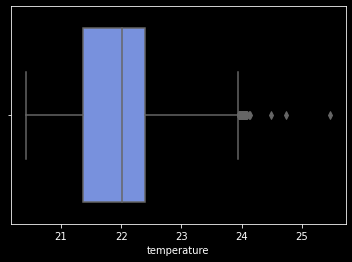
\includegraphics[width=0.90\textwidth]{univariate_3.png}
	\caption{Temperature boxplot}
\end{figure}

\subsection{Feature: Activity occupants}
We found that the Activity feature is heavily skewed towards no activities, putting it all together gives us a better distribution but we'll have to decide if we keep it exploded, put it together or remove it entirely.

\begin{figure}[H]
	\centering
	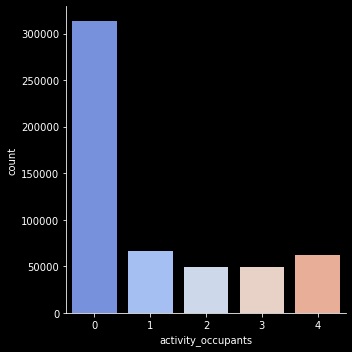
\includegraphics[width=0.90\textwidth]{univariate_4.png}
	\caption{Record count per activity}
\end{figure}

\subsection{Feature: Door state}
We found that the door state feature is heavily skewed towards the closed state. This needs to be considered when removing outliers.

\begin{figure}[H]
	\centering
	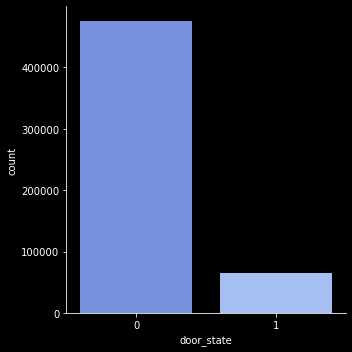
\includegraphics[width=0.90\textwidth]{univariate_5.png}
	\caption{Door state count per state}
\end{figure}

\subsection{Feature: Window state}
We found that the window state is completely unusable for our model because of its distribution.

\begin{figure}[H]
	\centering
	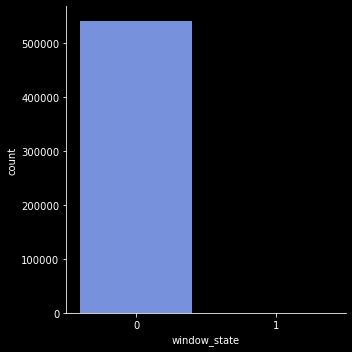
\includegraphics[width=0.90\textwidth]{univariate_6.png}
	\caption{Window state count per state}
\end{figure}



\section{Multivariate analysis}
With the discoveries from the univariate analysis we went forward with a multivariate analysis. 

\subsection{Feature: Room}
We found that when we plot the temperature and room feature together that there are a bunch of outliers in room 1. These will have to be removed in outlier removal.

\begin{figure}[H]
	\centering
	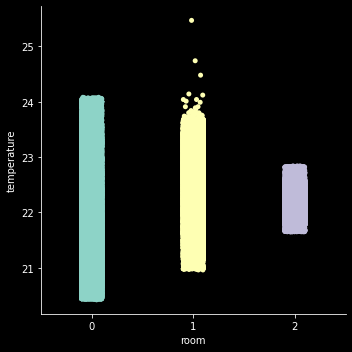
\includegraphics[width=0.90\textwidth]{bivariate_1.png}
	\caption{Record count per room}
\end{figure}

Next we plotted room on hour to see the distribution in records per room per hour.

\begin{figure}[H]
	\centering
	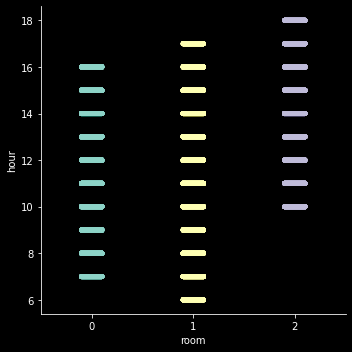
\includegraphics[width=0.90\textwidth]{bivariate_2.png}
	\caption{Record count per room}
\end{figure}

After that we also plotted the room and the mean-temp-day to see which records are from what year and what the mean temperature was that day. From this we can see a big difference in 2017 compared to 2016.

\begin{figure}[H]
	\centering
	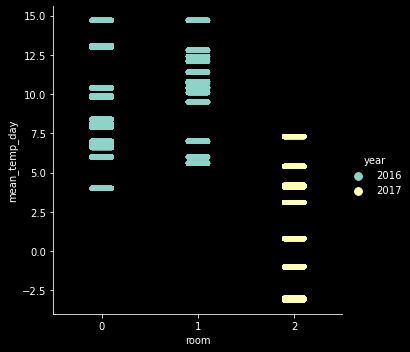
\includegraphics[width=0.90\textwidth]{bivariate_3.png}
	\caption{Record count per room}
\end{figure}

To confirm our suspicions about room 2 only having data from 2017 we plot the record count per year with hue being the room feature. From this we find that indeed room 2 only has data from 2017.

\begin{figure}[H]
	\centering
	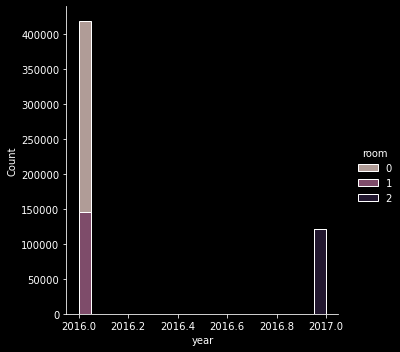
\includegraphics[width=0.90\textwidth]{bivariate_5.png}
	\caption{Record count per room}
\end{figure}

\subsection{Feature: Temperature}
We plotted temperature and meantemperature along with their bloxplots to see where the outliers lay. We found that most lay below 0 degrees meantemperature and above 24 degrees temperature.
\begin{figure}[H]
	\centering
	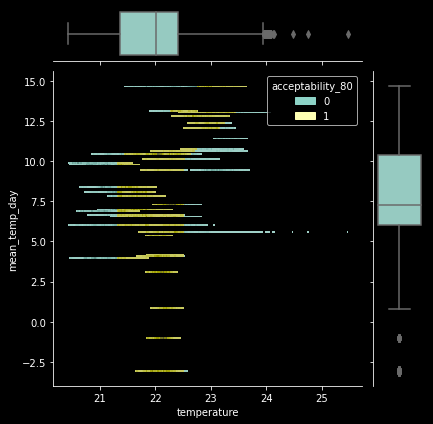
\includegraphics[width=0.90\textwidth]{bivariate_4.png}
	\caption{Record count per room}
\end{figure}

We wanted to plot temperature and heatindex to see if we have any outlying data. And indeed we have outlier data on the top end of heatindex and temperature.
\begin{figure}[H]
	\centering
	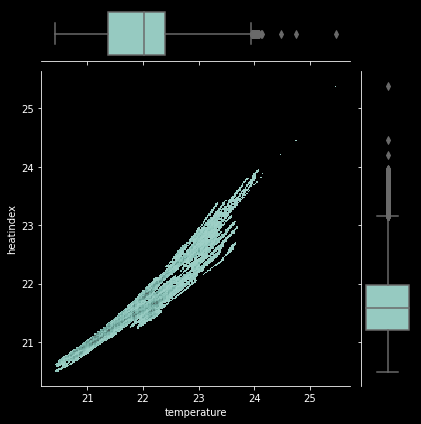
\includegraphics[width=0.90\textwidth]{bivariate_6.png}
	\caption{Record count per room}
\end{figure}

Too further confirm our suspicions on the temperature outliers we plot the temperature in a boxplot with year as hue. Furthermore we plotted that same data per room with the hue as year.
\begin{figure}[H]
	\centering
	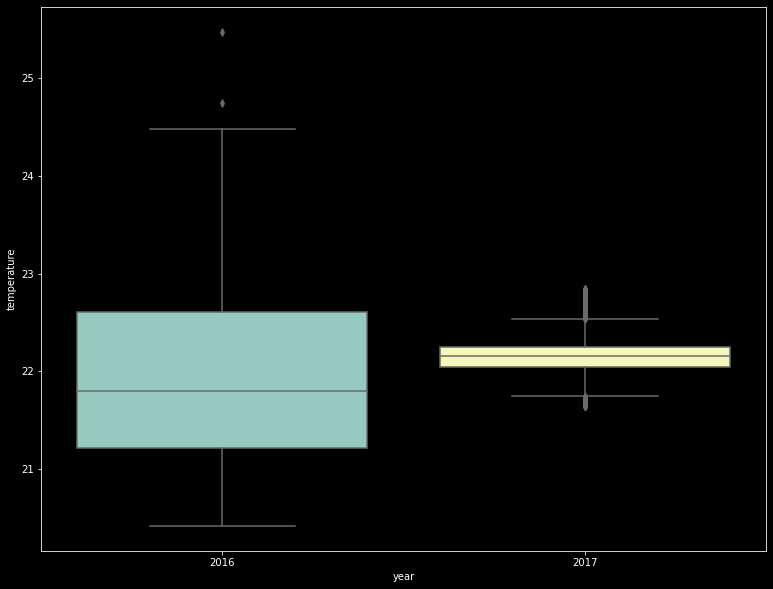
\includegraphics[width=0.90\textwidth]{bivariate_7.png}
	\caption{Record count per room}
\end{figure}

\begin{figure}[H]
	\centering
	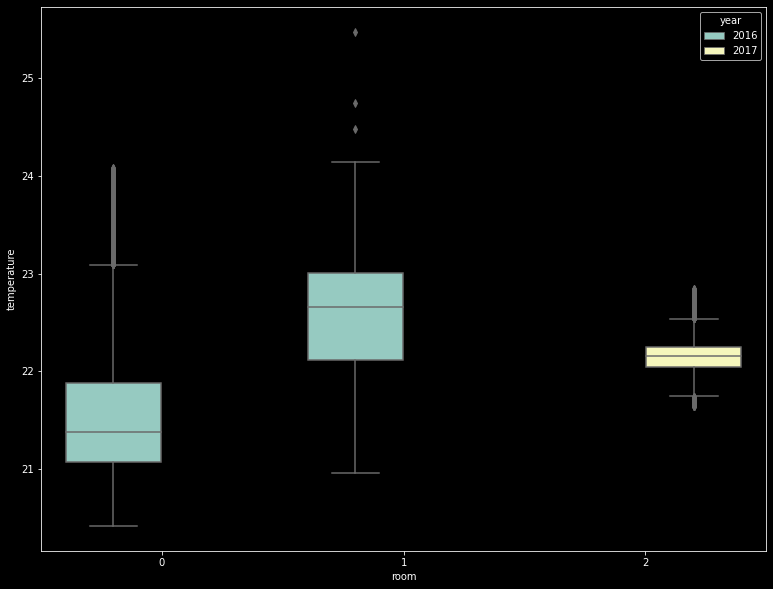
\includegraphics[width=0.90\textwidth]{bivariate_8.png}
	\caption{Record count per room}
\end{figure}


\end{document}
